%%%%%%%%%%%%%%%%%%%%%%%%%%%%%%%%%%%%%%%%%%%%%%%%%%%%%%%%%%%%%%%%%%%%%%%%%%%%%%%%
% AMS Beamer series / Bologna FC / Template
% Andrea Omicini
% Alma Mater Studiorum - Università di Bologna
% mailto:andrea.omicini@unibo.it
%%%%%%%%%%%%%%%%%%%%%%%%%%%%%%%%%%%%%%%%%%%%%%%%%%%%%%%%%%%%%%%%%%%%%%%%%%%%%%%%
%\documentclass[handout]{beamer}\mode<handout>{\usetheme{default}}
%
\documentclass[presentation, 8pt]{beamer}\mode<presentation>{\usetheme{AMSBolognaFC}}
%\documentclass[handout]{beamer}\mode<handout>{\usetheme{AMSBolognaFC}}
%%%%%%%%%%%%%%%%%%%%%%%%%%%%%%%%%%%%%%%%%%%%%%%%%%%%%%%%%%%%%%%%%%%%%%%%%%%%%%%%
\usepackage[T1]{fontenc}
\usepackage{wasysym}
\usepackage{amsmath,blkarray}
\usepackage{centernot}
\usepackage{fontawesome}
\usepackage{fancyvrb}
\usepackage{tasks}
\usepackage{minted}
\usepackage{listings}
\usepackage[ddmmyyyy]{datetime}
\renewcommand{\dateseparator}{}
\usemintedstyle{tango}
\setminted{frame=lines}
%\renewcommand{\thefootnote}{\fnsymbol{footnote}}
\newcommand{\version}{1}
\usepackage{xcolor}

\definecolor{dkgreen}{rgb}{0,0.6,0}
\definecolor{gray}{rgb}{0.5,0.5,0.5}
\definecolor{mauve}{rgb}{0.58,0,0.82}
\usepackage[
	backend=biber,
	citestyle=authoryear-icomp,
	maxcitenames=1,
	bibstyle=alphabetic]{biblatex}
\lstdefinestyle{scala}{
	language=scala,
	aboveskip=3mm,
	belowskip=3mm,
	showstringspaces=false,
	columns=flexible,
	basicstyle={\ttfamily},
	numbers=none,
	numberstyle=\tiny\color{gray},
	keywordstyle=\color{blue},
	commentstyle=\color{dkgreen},
	stringstyle=\color{mauve},
	breaklines=true,
	breakatwhitespace=true,
	tabsize=2,
}

\makeatletter
\addbibresource{biblio.bib}
%%%%%%%%%%%%%%%%%%%%%%%%%%%%%%%%%%%%%%%%%%%%%%%%%%%%%%%%%%%%%%%%%%%%%%%%%%%%%%%%
\title[Multi-Agent Reinforcement Learning]
{Multi-Agent Reinforcement Learning}
%
\subtitle[]
{on Collective Learning}
%
\author[\sspeaker{Aguzzi}]
{\speaker{Gianluca Aguzzi} \href{mailto:gianluca.aguzzi@unibo.it}{gianluca.aguzzi@unibo.it}}
%
\institute[DISI, Univ.\ Bologna]
{Dipartimento di Informatica -- Scienza e Ingegneria (DISI)\\\textsc{Alma Mater Studiorum} -- Universit{\`a} di Bologna}
%
\renewcommand{\dateseparator}{/}
\date[\today]{\today}

%
\AtBeginSection[]
{
  \begin{frame}
  \frametitle{Contents}
  \tableofcontents[currentsubsection, 
	sectionstyle=show/shaded, 
	subsectionstyle=show/shaded]
  \end{frame}
}
\AtBeginSubsection[]
{
  \begin{frame}
  \frametitle{Contents}
  \tableofcontents[currentsubsection, 
	sectionstyle=show/shaded, 
	subsectionstyle=show/shaded]
  \end{frame}
}
%
%%%%%%%%%%%%%%%%%%%%%%%%%%%%%%%%%%%%%%%%%%%%%%%%%%%%%%%%%%%%%%%%%%%%%%%%%%%%%%%%
\begin{document}
%%%%%%%%%%%%%%%%%%%%%%%%%%%%%%%%%%%%%%%%%%%%%%%%%%%%%%%%%%%%%%%%%%%%%%%%%%%%%%%%

%/////////
\frame{\titlepage}
%/////////

%%===============================================================================
\section*{Outline}
%%===============================================================================

%===============================================================================
\section{Introduction}
%===============================================================================

%/////////
\begin{frame}[c]{Multi-Agent Reinforcement Learning (MARL)}
%/////////

\begin{exampleblock}{Definition}
	\emph{Multiple} agents \textbf{learn} to take the \emph{right} actions (\textbf{policy}) to maximise a \emph{reward} signal (collective, selfish, \dots).
\end{exampleblock}

\begin{alertblock}{Applications}
	\begin{tasks}(2)
		\task Videogames
		\task Trafic Control
		\task Robotics (\emph{Swarm robotics})
		\task Trading
		\task Energy Management
		\task Environmental Monitoring
	\end{tasks}
\end{alertblock}
\begin{exampleblock}{Today Outline}
	\begin{itemize}
		\item MARL abstractions
		\begin{itemize}
			\item[\faArrowRight] From MDP to Stochastic game
		\end{itemize}
		\item MARL classification
		\begin{itemize}
			\item[\faArrowRight] Cooperative vs. Competitive agents
			\item[\faArrowRight] Centralised vs Decentralised learning and acting
			\item[\faArrowRight] Homogeneous vs Heterogeneous agents
		\end{itemize}
		\item MARL learning algorithms 
		\item Scale to \textbf{infinity}: MARL in Collective Adaptive Systems \& Aggregate Computing
	\end{itemize}
\end{exampleblock}
\end{frame}
\begin{frame}{Motivating Example}
\centering
\begin{exampleblock}{OpenAI Hide And Seek: \url{https://openai.com/blog/emergent-tool-use/}}
	\begin{figure}
		\href{https://www.youtube.com/watch?v=kopoLzvh5jY}{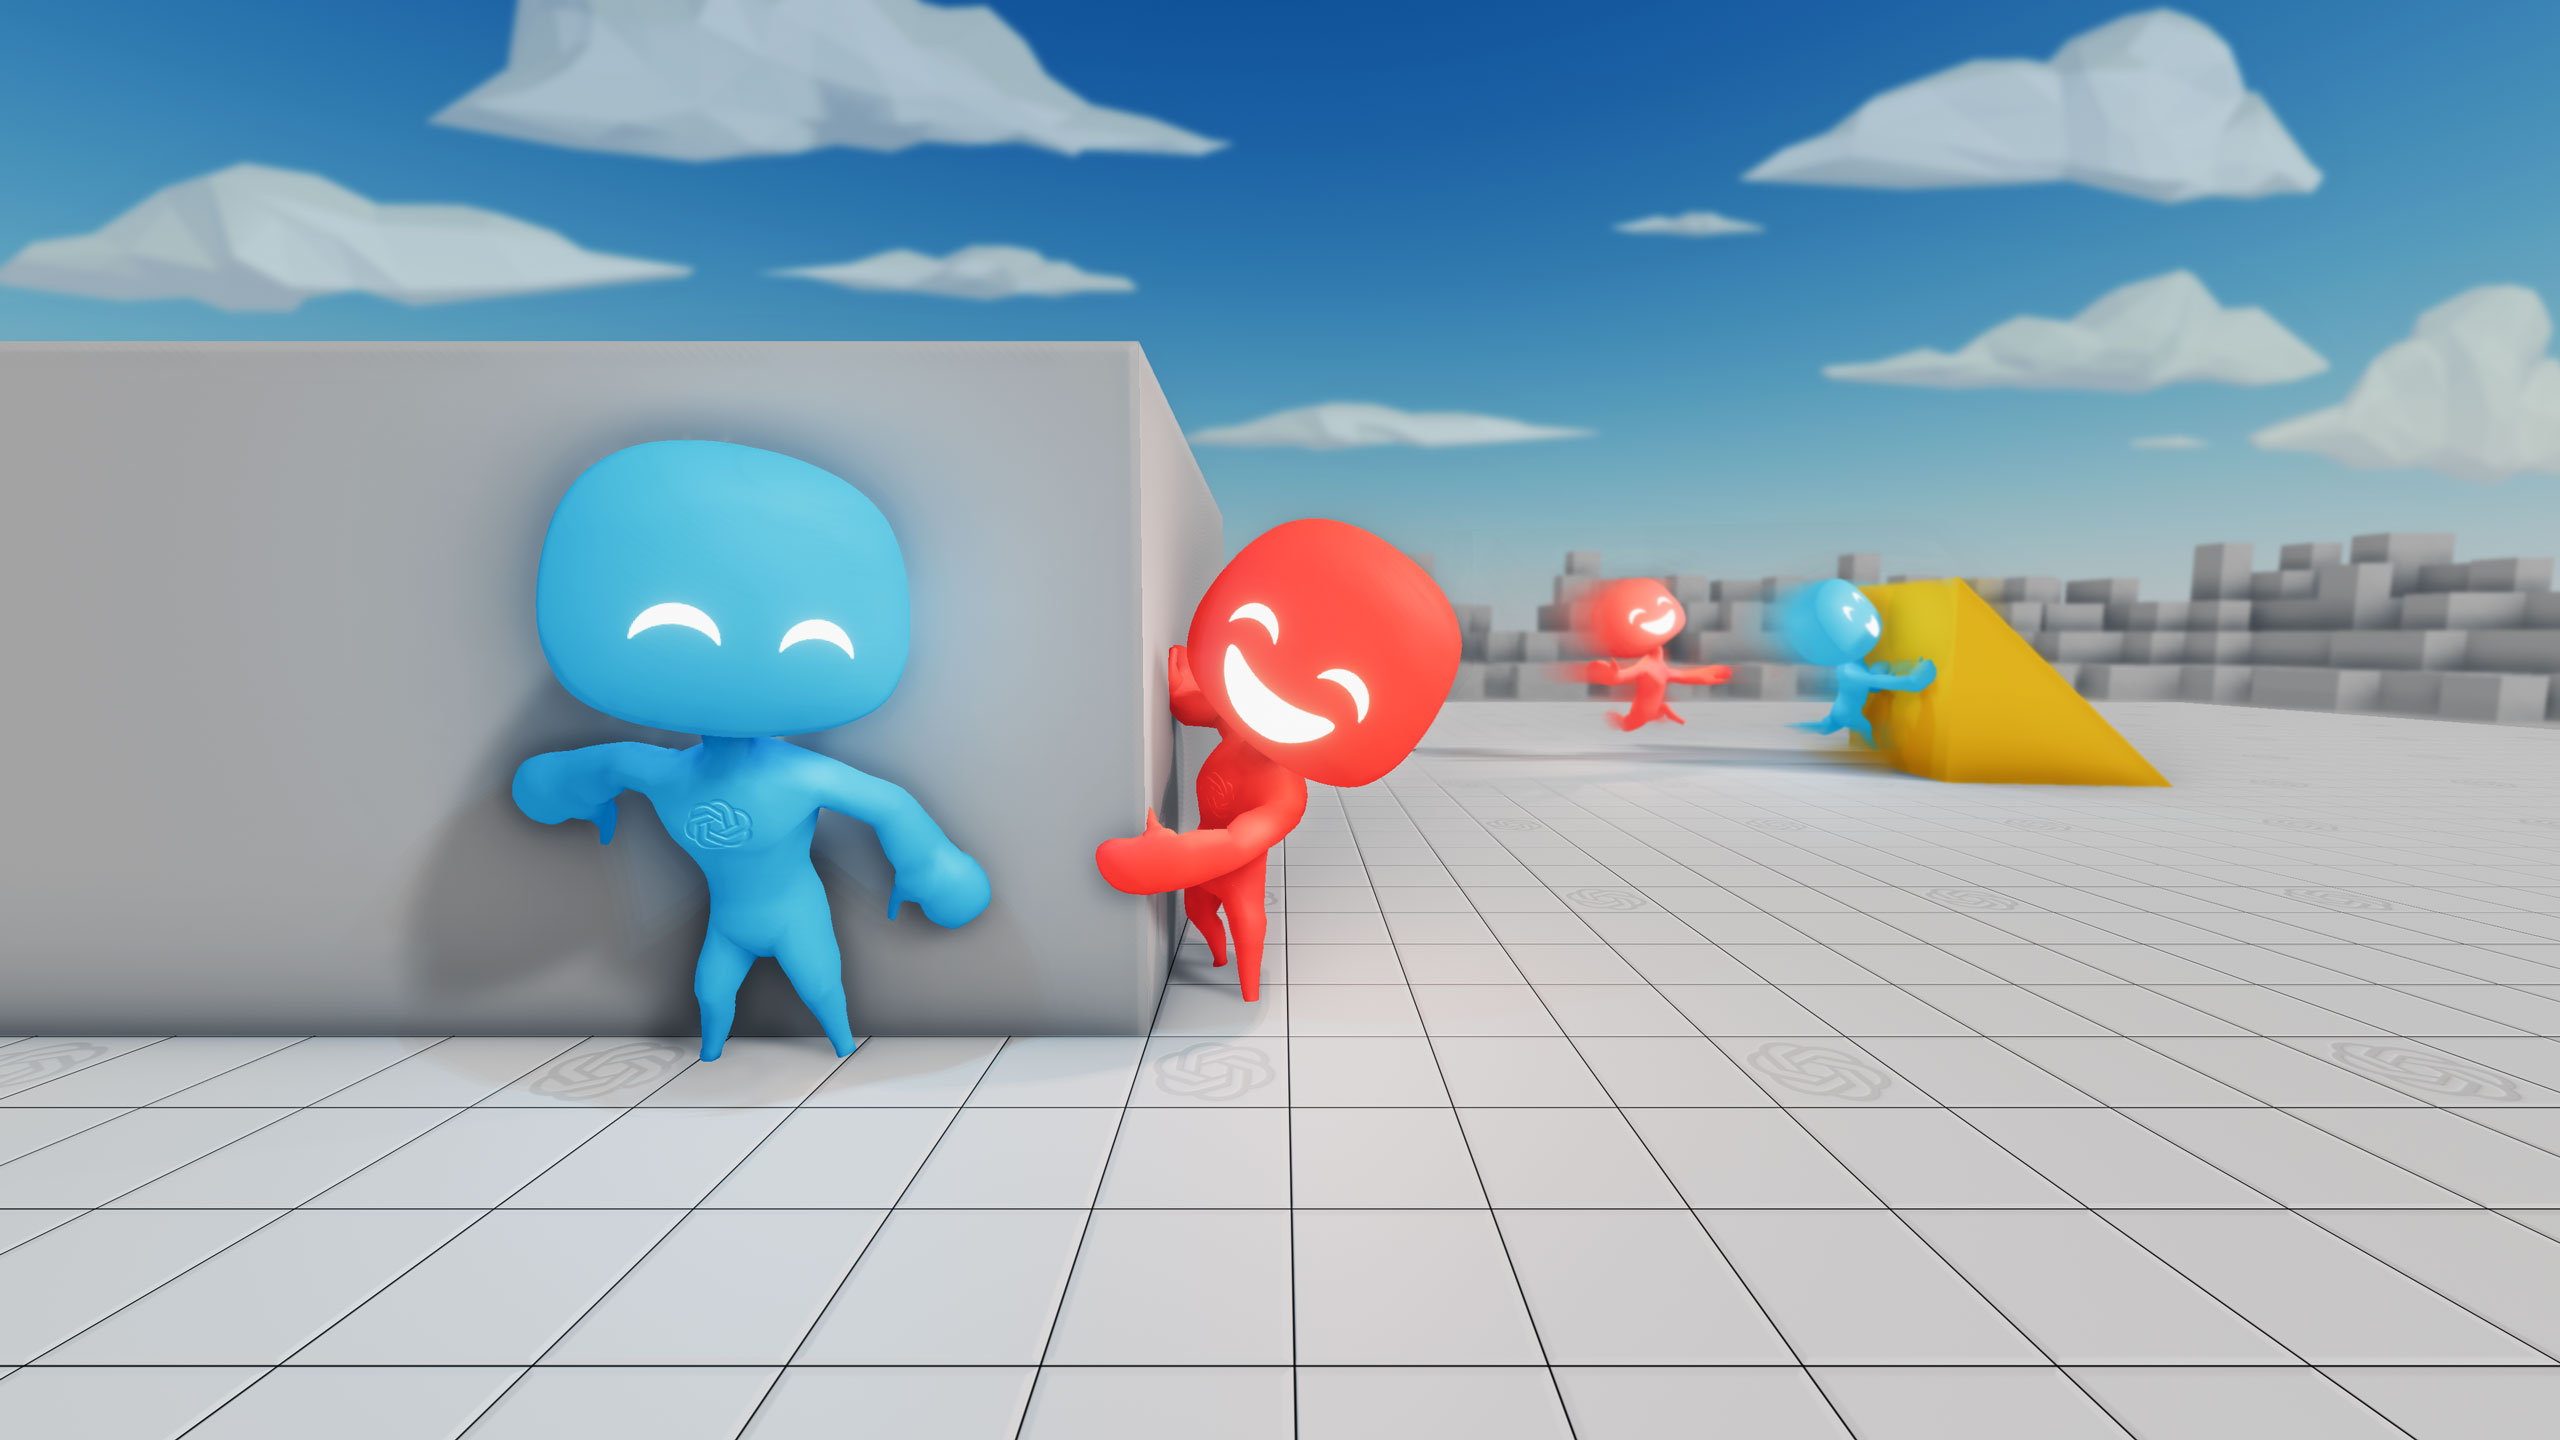
\includegraphics[width=\textwidth]{img/open-ai.jpg}}
	\end{figure}
\end{exampleblock}
\end{frame}
\subsection{Stochastic Games}
%/////////
\begin{frame}[c]{Stochastic Game $\mathcal{S}$ (or Markov games)}
	%/////////
	\begin{alertblock}{Definition}
		\begin{itemize}
			\item $\mathcal{S}$ is a tuple $<N, S, \{A^i\}_{i \in \{ 1, \dots, N\}}, P, \{R^i\}_{i \in \{ 1, \dots, N\}}>$
			\item $N$ is the number of agents ($|N| > 1 $)
			\item $S$ is the global environment state
			\item $A^i$ is the action state of agent $i$. $\mathbb{A} := A^1 \times \dots\times A^N$ is the joint action space
			\item $P: S x \mathbb{A} \rightarrow \mathcal{P}(S)$ is the state transaction. $\mathcal{P}$ is a discrete probabilistic distribution %(associate for each $s \in S$ a probability)
			\item $R^i: S \times \mathbb{A} \times S \rightarrow \mathbb{R}$ is the reward signal
			\item Typical time evolution: $ S_0, \mathbb{A}_0, \mathbb{R}_1, S_1, \dots  $
		\end{itemize}
	\end{alertblock}
	\begin{exampleblock}{Paper Rock Scissor (Repeated)}
		\begin{tasks}(2)
			\task $N = 2$
			\task $A^1 = A^2 = $ \{Paper, Rock, Scissor\}
			\task $S = \{ \mathbb{A}_{t-1} \} $
			\task $R = \begin{blockarray}{cccc}
        & Rock & Paper & Scissor \\
      \begin{block}{c[ccc]}
        Rock    & 0, 0  & -1, 1 & 1, -1 \\
        Paper   & 1, -1 & 0, 0  & -1, 1 \\
        Scissor & -1, 1 & 1, -1 & 0, 0 \\
      \end{block}
    \end{blockarray}$
		\end{tasks}
	\end{exampleblock}
\end{frame}	
\begin{frame}[fragile, allowframebreaks]{Stochastic Game (Scala Modelling)}
\begin{exampleblock}{Stochastic Game Model}
\begin{lstlisting}[style=scala]
trait StochasticGame[State, Action]:
	def agents: Int 
	def initialState: Distribution[State]
	def transitionFunction: (State, Seq[Action]) => Distribution[State]
	def rewardFunction: (State, Seq[Action], State) => Seq[Double]
\end{lstlisting}	
\end{exampleblock}
\begin{exampleblock}{Multi-Agent Environment façade}
	\begin{lstlisting}[style=scala]
trait MultiAgentEnvironment[State, Action]:
	// current environment state
	def state: State
	// given a joint action, return the reward
	def act(actions: Seq[Action]): Seq[Double]
	// reset the internal environment state 
	def reset(): Unit 
\end{lstlisting}	
\end{exampleblock}
\begin{exampleblock}{Environment factory}
\begin{lstlisting}[style=scala]
object StochasticGame:
	def createEnvironment[State, Action](
			stochasticGame: StochasticGame[State, Action]
	): MultiAgentEnvironment[State, Action] =
		new MultiAgentEnvironment: // hide the dynamics on a MAS facade
			var state: State = stochasticGame.initialState.sample
			override def act(actions: Seq[Action]): Seq[Double] =
				val previousState = state
				val nextState = stochasticGame.transitionFunction(state, actions)
				state = nextState.sample
				stochasticGame.rewardFunction(previousState, actions, state)
			override def reset(): Unit = state = stochasticGame.initialState.sample
\end{lstlisting}
\end{exampleblock}
\begin{exampleblock}{Repeated Rock Paper Scissor}
\begin{lstlisting}[style=scala]
class Dynamics extends StochasticGame[State, Action]:
	override def agents: Int = 2

	override def initialState: Distribution[State] =
		Distribution.one(Seq(None, None))
	override def transitionFunction: (State, Seq[Action]) => Distribution[State] =
		(_, actions) => Distribution.one(actions.map(Some(_)))

	override def rewardFunction: 
		(State, Seq[Action], State) => Seq[Double] = (_, actions, _) => payoff(actions.toList)

	private def payoff(actions: List[Choice]): Seq[Double] = actions match
		case left :: right :: Nil if left == right => List(0, 0)
		case Rock :: Scissor :: Nil => List(1, -1)
		case Scissor :: Paper :: Nil => List(1, -1)
		case Paper :: Rock :: Nil => List(1, -1)
		case left :: right :: Nil =>
			payoff(right :: left :: Nil).reverse
\end{lstlisting}
\end{exampleblock}
\end{frame}
\section{Learning in Multi Agent Environment}
\begin{frame}[allowframebreaks]{Learning in Multi Agent Environment / Stochastic Games}
\begin{exampleblock}{Task type}
	\begin{itemize}
		\item \textbf{Cooperative}
		\begin{itemize}
			\item Agents share the same reward function ($R^1 = R^2 = \dots = R^N$) or the same collective goal
			\item Examples: multi-agent pathfinding, multi-agent resource allocation, multi-agent task allocation, \dots
		\end{itemize}
		\item \textbf{Competitive}
		\begin{itemize}
			\item Agents compete with each other to maximise a long-term return
			\item Examples: Boards games, battle games, \dots
		\end{itemize}
	\end{itemize}
\end{exampleblock}
%%%%
\begin{exampleblock}{Policy Type}
\begin{itemize}
	\item \textbf{Homogeneous}
	\begin{itemize}
		\item Each agent has the same action space ($ A^1 = A^2 = .. A ^N$) and use the \textbf{same} policy ($ \pi^0 = \pi^N$)
		\item Used in \emph{cooperative} settings and with many agent interactions (e.g., swarm robotics)
		\begin{itemize}
			\item Complexity emerges from interactions
		\end{itemize}
		\item Examples (swarm robotics): obstacle avoidance, flocking, team formation, \dots
	\end{itemize}
	\item \textbf{Heterogeneous}
	\begin{itemize}
		\item Each agent has a different action space ($ A^1 \neq A^2 \neq .. A ^N$) and use a \textbf{different} policy ($ \pi^0 \neq \pi^N$)
	\end{itemize}
\end{itemize}
\end{exampleblock}
%%%%
\begin{exampleblock}{Communication constraints}
\begin{itemize}
	\item \textbf{Independent}
	\begin{itemize}
		\item The policy of each agent is independent of the policy of the other agents
		\item Cooperation could emerge through environment dynamics (but is hard)
	\end{itemize}
	\item \textbf{Joint Action}
	\begin{itemize}
		\item The policy of each agent depends on the action of the other agents ($ \pi(s_t, a^{-i}_t)^i $, where $-i$ means the other agents' indices)
		\item Cooperation is explicitly encoded in the policy
		\item Action space exponentially increases with the agent population
	\end{itemize}
\end{itemize}
\end{exampleblock}
%%%%
\begin{exampleblock}{Execution constraints}
\begin{itemize}
	\item \textbf{Centralised}
	\begin{itemize}
		\item A central controller is responsible for the execution of the policy
		\item It has a global view of the environment and can coordinate the agents
	\end{itemize}
	\item \textbf{Decentralised}
	\begin{itemize}
		\item Each agent executes its own policy
		\item They don't have a global view of the environment, but (potentially) they can communicate
	\end{itemize}
\end{itemize}
\end{exampleblock}
%%%%
\begin{exampleblock}{Learning constraints}
\begin{itemize}
	\item \textbf{Centralised}
	\begin{itemize}
		\item A central agent is responsible for the learning process
		\item It could produce centralised or decentralised policies
	\end{itemize}
	\item \textbf{Decentralised}
	\begin{itemize}
		\item Each agent has its own learning process
		\item It mainly produces decentralised policies
	\end{itemize}
\end{itemize}
\end{exampleblock}

\begin{alertblock}{Big Question: Can we use Single Agent RL in MAS?}
\begin{itemize}
	\item It depends on the \emph{task type}, \emph{policy type}, \emph{communication} constraints, \emph{execution} constraints, and \emph{learning} constraints
	\item Single agent RL could be easily adapted in some cases:
	\begin{itemize}
		\item Task type: cooperative
		\item Policy type: homogeneous
		\item Communication constraints: independent
		\item Execution constraints: centralised/decentralised
		\item Learning constraints: centralised/decentralised
	\end{itemize}
	\item In other cases, they could fail easier
\end{itemize}
\end{alertblock}
\end{frame}
\begin{frame}[fragile, allowframebreaks]{Learning in MAS: Abstractions}
\begin{exampleblock}{Agent Definition}
	\begin{itemize}
		\item An agent is a function that maps an observation to an action
		\item Observation could be different from environment state (i.e., the agent could have a different view of the environment)
		\item It records the trajectory of the agent-environment interactions $(s, a, r, s')$ 
	\end{itemize}
\begin{lstlisting}[style=scala]
trait Agent[-Obs, Action]:
	def act(state: Obs): Action
	def record(state: Obs, action: Action, reward: Double, nextState: Obs): Unit 
	def reset(): Unit
\end{lstlisting}
\end{exampleblock}
\begin{exampleblock}{Learner extension}
\begin{itemize}
	\item A \lstinline[style=scala]{Learner} is a special type of agent that has a policy that will be improved through experience
	\item It has two policy, \emph{behavioural} used during the training, and \emph{optimal} used to test the agent
\end{itemize}
\begin{lstlisting}[style=scala]
trait Learner[Obs, Action]:
  self: AI.Agent[Obs, Action] =>
	def mode: AgentMode
  def optimal: Obs => Action // used to test the agent
  def behavioural: Obs => Action // used during training
  override def act(state: Obs): Action = 
		(if mode == AgentMode.Training then behavioural else optimal) (state)
	override def record(
		state: Obs, action: Action, reward: Double, nextState: Obs
	): Unit =
    if mode == AgentMode.Training then improve(state, action, reward, nextState)
  def improve(state: Obs, action: Action, reward: Double, nextState: Obs): Unit
\end{lstlisting}
\end{exampleblock}
\framebreak
\begin{exampleblock}{Q Learner Implementation}
	\begin{lstlisting}[style=scala]
class QAgent[Obs, Action: Enumerable](
		q: Q[Obs, Action], alpha: Ref[Double], gamma: Double, epsilon: Double
)(using random: Random) extends Agent[Obs, Action] with Learner[Obs, Action]:
	val optimal: Obs => Action = state => bestOutcome(state)._1 // Greedy policy
	val behavioural: Obs => Action = state => // Epsilon greedy policy
		if random.nextDouble() < epsilon.value 
			then random.shuffle(Enumerable[Action]).head
			else optimal(state)

	override def improve(....): Unit =
		val qT = q(state, action)
		val (_, qMax) = bestOutcome(nextState)
		val update = qT + alpha.value * (reward + gamma * qMax - qT)
		q.update(state, action, update)

	private def bestOutcome(state: Obs): (Action, Double) =
		Enumerable[Action].map(action => (action, q(state, action))).maxBy(_._2)

	\end{lstlisting}
\end{exampleblock}

\begin{exampleblock}{Simulation definition}
	\begin{lstlisting}[style=scala]
class Simulation[State, Action](
	val environment: MultiAgentEnvironment[State, Action]
):
	def simulate(
		episodes: Int, episodeLength: Int, agents: Seq[Agent[State, Action]]
	): Unit =
		for episode <- 0 to episodes do
			agents.foreach(_.reset())
			environment.reset()
			for _ <- 0 to episodeLength do
				val currentState = environment.state
				val actions = agents.map(_.act(currentState))
				val rewards = environment.act(actions)
				val nextState = environment.state
				val actionAndRewards = actions.zip(rewards)
				agents.zip(actionAndRewards).foreach { case (agent, (action, reward)) =>
					agent.record(currentState, action, reward, nextState)
				}
\end{lstlisting}
\end{exampleblock}
\end{frame}
\subsection{Learning in Competitive Multi Agent Environment}
\begin{frame}{Learning in Competitive Multi Agent Environment: Repeated Rock Paper Scissors}
	\begin{alertblock}{Goal?}
		\begin{itemize}
			\item An agent always wins against a random agent?
			\item An agent always wins against a fixed strategy agent?
			\item An agent always wins against a learning agent?
			\item Nash equilibrium: no agent can improve its performance by changing its strategy
		\end{itemize}
	\end{alertblock}
	\begin{exampleblock}{Repeated Rock Paper Scissor Example}
		\begin{itemize}
			\item Nash equilibrium: all agents play randomly
			\item In this case: 
			\begin{itemize}
				\item With Q-Learning we will find deterministic strategies
				\item The equilibrium will reach a condition in which each play always plays the same action
			\end{itemize}
		\end{itemize}
	\end{exampleblock}
\end{frame}
\subsection{Learning in Cooperative Multi Agent Environment}
\begin{frame}[allowframebreaks]{Learning in Cooperative Multi Agent Environment: Agents Alignment}
\begin{exampleblock}{Agents Alignment}
	\begin{itemize}
		\item \textbf{N} Agents live in a bounded grid world of size $W \times H$
		\item Each agent has a position in the grid $(x_i, y_i)$
		\item The state of the environment consists in the position of all the agents $X = {(x_1, y_1), (x_2, y_2), ..., (x_n, y_n)}$
		\item The action of each agent is one of the following (up, down, left, right, stay)
		\item Collective goal: all agents should be aligned in the same row/column
		\begin{itemize}
			\item reward function: if all agents are aligned, then reward = 10, otherwise reward = -1
		\end{itemize}
	\end{itemize}
\end{exampleblock}
\centering
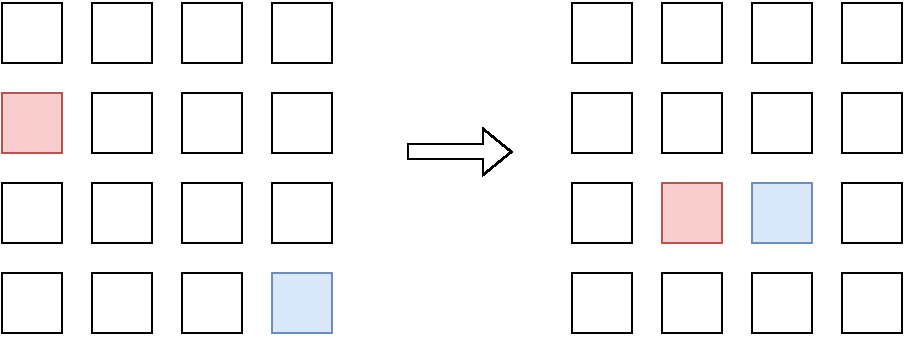
\includegraphics[width=0.8\textwidth]{img/agent-modelling.pdf}
\begin{alertblock}{How?}
	\begin{itemize}
		\item Independent Learner with Heterogeneous Policy
		\begin{itemize}
			\item Each agent has its own policy and Q table
			\item They update it during the training
			\item \textbf{Problems}:
			\begin{itemize}
				\item Non-stationary environment (the state of the environment changes during the training)
				\item It hardly scales with the number of agent
			\end{itemize}
		\end{itemize}
		\item Centralised Learner with Homogeneous Policy
		\begin{itemize}
			\item Each agent has access to a shared Q-table and policy
			\item That table is updated during the training
			\item \textbf{Problems}:
			\begin{itemize}
				\item The policy is simpler with the respect to the one of the independent learners
				\item \dots but it potentially scales with any number of agents
			\end{itemize}
		\end{itemize}
		\item Centralised Learner with Centralised and Joint Policy
		\begin{itemize}
			\item A central server coordinates the training and the execution of the agents
			\item The server has a policy and a Q-table that depends on the joint action of all the agents
			\item \textbf{Problems}:
			\begin{itemize}
				\item The action space grows exponentially with the number of agents (e.g. 5 agents, 5 actions each, $5^5=3125$ possible joint actions)
			\end{itemize}
		\end{itemize}
		\item NB! Tabular methods are not the only ones that can be used to solve this problem \faArrowRight \, \textbf{Deep Reinforcement Learning} for complex state environment (o partial observable state)
	\end{itemize}
\end{alertblock}
\end{frame}
\subsection{Introduction on Deep Reinforcement Learning}

\begin{frame}{Introduction of Deep Reinforcement Learning}
\begin{itemize}
	\item Tabular Reinforcement Learning (e.g., Q Learning, SARSA, ...) has several limitations:
	\begin{itemize}
		\item It is not able to handle complex state space 
		\begin{itemize}
			\item Agent Alignment example: state space size is equal to: $(WxH)^N$
			\begin{tasks}
				\task $W = H = 5$, $N = 2$ = $25^2$ = 625
				\task $W = H = 5$, $N = 3$ = $25^3$ = 15625
				\task $W = H = 5$, $N = 4$ = $25^4$ = 390625
			\end{tasks}
		\end{itemize}
		\item It is not able to handle partial observable state space
		\item It is not able to handle continuous action space
		\item \dots
	\end{itemize}
	\item Deep Reinforcement Learning is a family of methods that overcome these limitations using \emph{neural networks}
	\item Several algorithms have been proposed:
	\begin{itemize}
		\item \textbf{Deep Q-Learning}: The Q-table is approximated by a neural network
		\begin{itemize}
			\item It could handle continuous state space
			\item It could be used for raw input (e.g., images)
			\item It has been used to solve complex tasks (e.g., Atari games)
		\end{itemize}
		\item Policy Gradient: the neural networks are used to represent the \emph{policy} of the Agents
		\item Several others: Actor-Critic, Deep Deterministic Policy Gradient, \dots
	\end{itemize}
\end{itemize}
\end{frame}
\begin{frame}[allowframebreaks, fragile]{Deep Q-Learning}
	\begin{exampleblock}{Key ingredients}
		\begin{itemize}
		\item \textbf{network network}: A neural network that maps the state to the action/value pairs.
		\begin{itemize}
			\item It could be seen as a function from state to (action, value) pairs. 
		\end{itemize}
		\item \textbf{target network}: It has the same architecture of the network policy, but is used to compute the target value.
		\begin{itemize}
			\item the target policy is updated less frequently than the network policy, to improve the stability of the learning process.
		\end{itemize}
		\item \textbf{reply buffer/experience replay}: It is used to store the experience of the agent during the training.
		\begin{itemize}
			\item This experience is then used to train the network policy.
			\item The experience is sampled randomly from the buffer.
			\begin{itemize}
				\item this reduces the correlation between the samples.
			\end{itemize}
		\end{itemize}
	\end{itemize}
	\end{exampleblock}
	\centering
	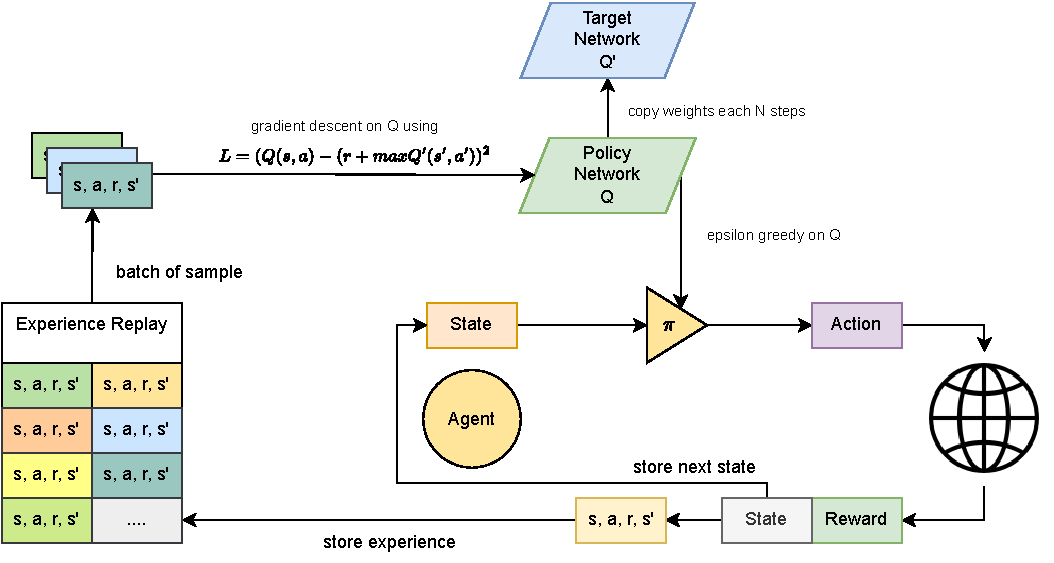
\includegraphics[width=\textwidth]{img/dqn.pdf}
	\begin{exampleblock}{Pseudocode}
\begin{lstlisting}[style=scala]
val policyNetwork = // initialize the network policy
val targetNetwork = // initialize the target network
val replyBuffer = // initialize the reply buffer
for(episode <- 1 to maxEpisodes) do
	val environment = // initialize the environment
	for(step <- 1 to maxSteps) do
		val action = policyNetwork(state)
		val (nextState, reward) = environment.execute(action)
		replyBuffer.add(state, action, reward, nextState)
		val batch = replyBuffer.sample(batchSize)
		val targetValue = batch.map { experience =>
			val (state, action, reward, nextState) = experience
			val targetValue = reward + discountFactor * targetNetwork(nextState)
		}
		policyNetwork.update(batch, targetValue)
		if(step % targetNetworkUpdateFrequency == 0) then
			targetNetwork = policyNetwork
		
\end{lstlisting}
	\end{exampleblock}
\end{frame}
\section{Scale to \textbf{Infinity}: Learning in CAS}
\begin{frame}{Learning in CAS}
	\begin{alertblock}{Problems}
		\begin{itemize}
			\item Collective Adaptive System are challenging environments for learning
			\begin{itemize}
				\item The agents involved could be hundreds or thousands
				\item The state space could be very large
				\item The agents only have partial information about the state
				\item No central controller (at runtime)
			\end{itemize}
		\end{itemize}
	\end{alertblock}
	
	\begin{alertblock}{How?}
		\begin{itemize}
			\item Constraints on policy: \emph{homogeneous}
			\begin{itemize}
				\item The \textbf{complexity} emerges through interactions
			\end{itemize}
			\item Partial observability handled through \emph{deep learning} (e.g., Deep Q-Learning)
			\item Centralised training and decentralised execution strategy
			\begin{itemize}
				\item During the simulation the agents are trained using a centralised training algorithm
				\item The Q table is local to each agent
				\item After the simulation, it will be copied into each agent
				\item No need for a central controller at runtime!
			\end{itemize}
			\item Communication handled through \emph{message passing} and encoded as a local state
			\item \emph{Dense} reward to simplify the learning process and to enable cooperation
		\end{itemize}
	\end{alertblock}
\end{frame}
\begin{frame}{Example: Simple Flocking Behaviour}
	\begin{exampleblock}{Scenario}
		\begin{itemize}
			\item \textbf{N} agents placed in a 2D world
			\item Each agent has \textbf{M} neighbours
			\item The action spaces is the set of possible directions (e.g., 8 directions + stand still)
			\item The state space is the set distance vector to the neighbours
			\begin{itemize}
				\item State space size: \emph{M * 2}
			\end{itemize}
			\item Goal: the agents should move without colliding and try to stay close to each other
			\item reward function is composed of two te
			\begin{itemize}
				\item cohesion: the farthest agent distance should be as small as possible
					\begin{itemize}
						\item $R_cohesion = -(max_{distance} - target_{distance})$
					\end{itemize}
				\item collision: the nearest agent distance should be as large as possible
				\begin{itemize}
					\item $R_collision = log(min_{distance} / target_{distance})$
				\end{itemize}
			\end{itemize}
		\end{itemize}
	\end{exampleblock}
\end{frame}
\subsection{Hybrid Aggregate Computing}
\begin{frame}{Hybrid Aggregate Computing}
	\begin{alertblock}{Why}
		\begin{itemize}
			\item \textbf{Aggregate Computing}: framework used to express self-organising behaviours
			\begin{itemize}
				\item[\faThumbsUp] Flexible and expressive
				\item[\faThumbsUp] Scalable to a large number of agents
				\item[\faThumbsUp] Robust to failures
			\end{itemize}
			\item Limitations:
			\begin{itemize}
				\item Distributed Algorithms typically involve fine-tuning made by experts
				\item Certain behaviours are difficult to express
				\item Adaptive behaviours could be hard to implement
				\item \faArrowRight \, ML could be a mechanism to overcome these limitations
			\end{itemize}
		\end{itemize}
	\end{alertblock}
	\begin{alertblock}{Where?}
		\begin{itemize}
			\item \textbf{Algorithms definition}: RL could be employed to learn part of aggregate algorithms 
			\begin{itemize}
				\item[\faArrowRight] \citefield{aguzzi2022towards}{title}
			\end{itemize}
			\item \textbf{Execution strategy}: For the same program, several execution strategies could carry on the right result. RL could be used to learn the best strategy that improves the performance of the system 
			\begin{itemize}
				\item[\faArrowRight] \citefield{aguzzi2022addressing}{title}
			\end{itemize}
			\item \textbf{System structure}: RL could be used to learn the best structure (i.e., where to \emph{place} the computation) of the system.
		\end{itemize}
	\end{alertblock}
\end{frame}

\begin{frame}{Example: Follow the leader}
\begin{exampleblock}{Scenario}
	\begin{itemize}
		\item Same setting as before (N agents, M neighbours, 8 directions + stand still)
		\item But aggregate computing is used to share the leader towards a gradient
		\item Reward function is composed of two terms
		\begin{itemize}
			\item collision: the nearest agent distance should be as large as possible (same as before)
			\item leader: the distance to the leader should be as small as possible
		\end{itemize}
	\end{itemize}

\end{exampleblock}
\centering {
	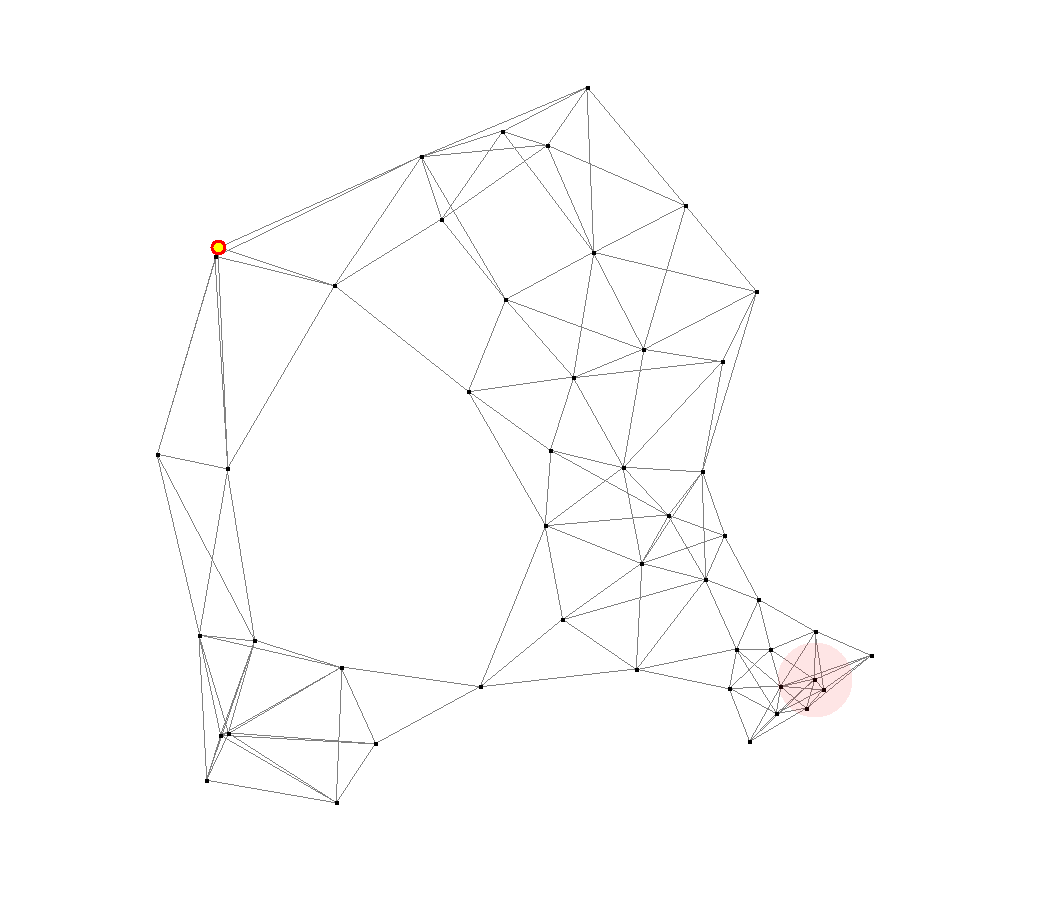
\includegraphics[width=0.3\textwidth]{img/moment-a.png}
	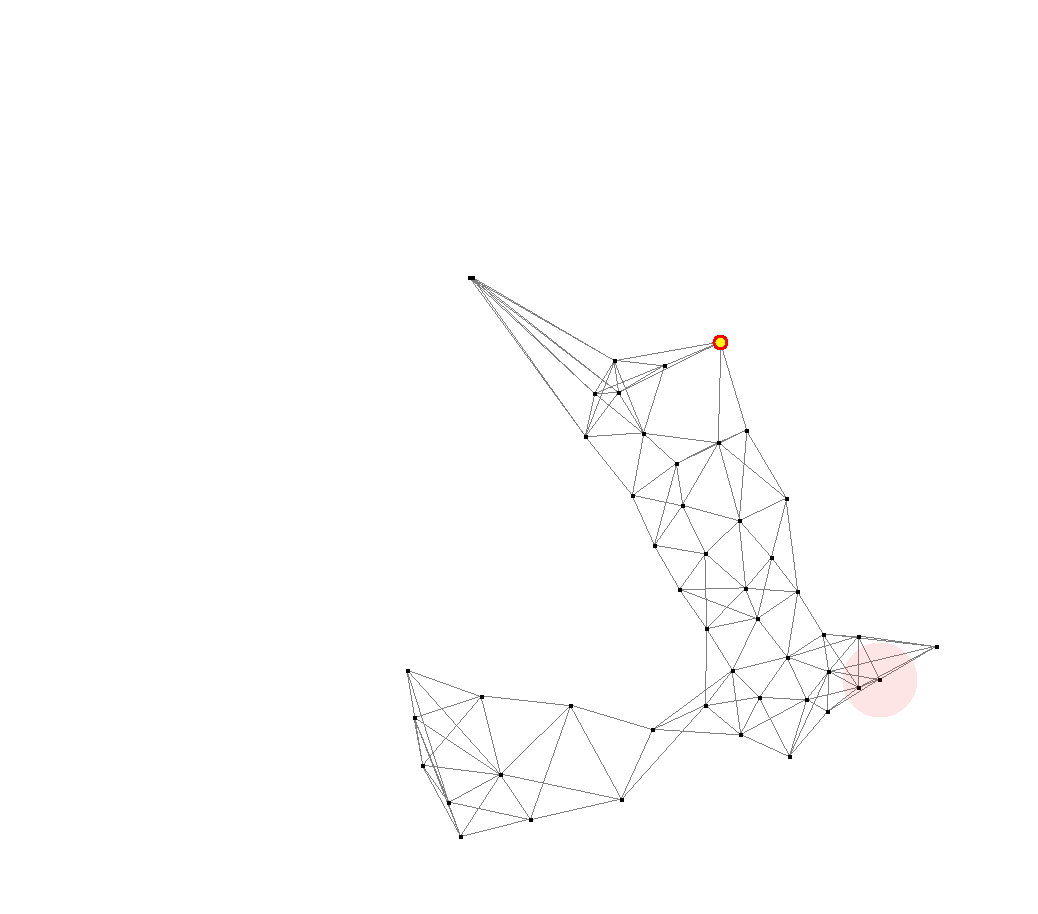
\includegraphics[width=0.3\textwidth]{img/moment-b.png}
	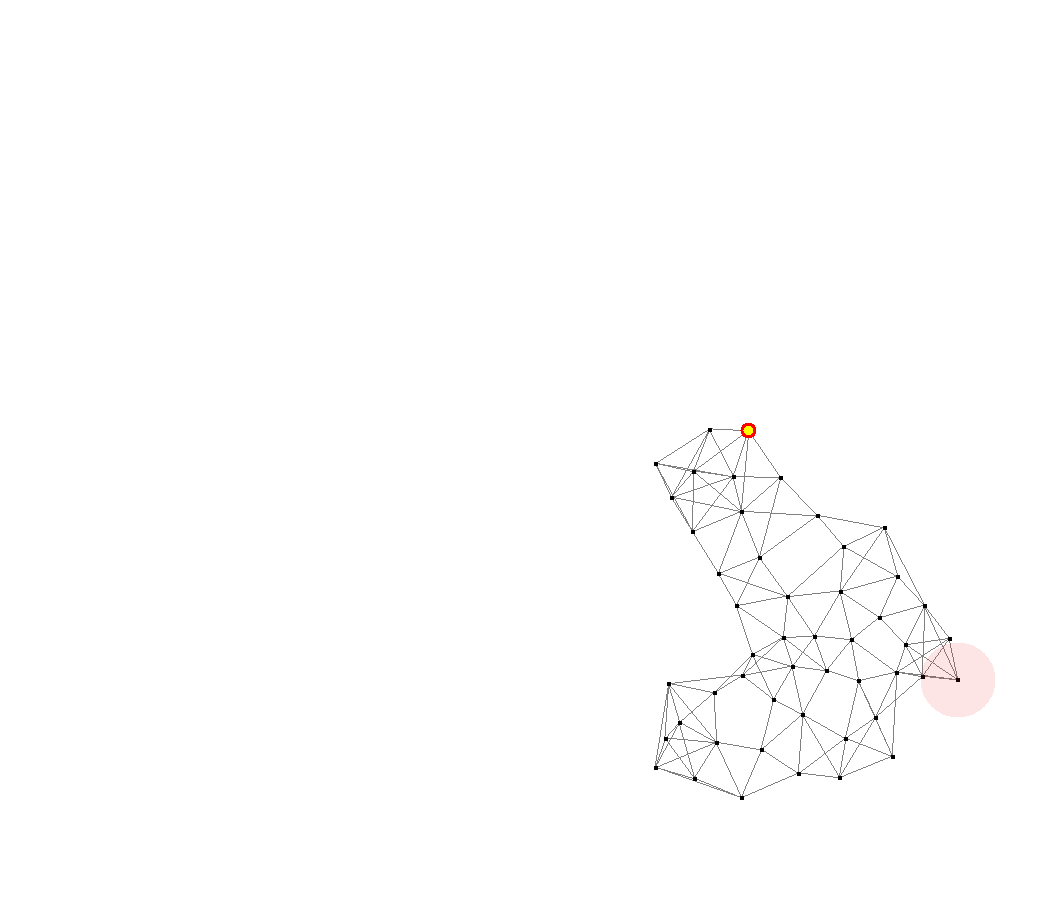
\includegraphics[width=0.3\textwidth]{img/moment-c.png}
}
\end{frame}

\begin{frame}{Conclusion}
\begin{itemize}
	\item Aggregate computing \faPlus \, ML is still an open research area
	\item Preliminary results are promising ...
	\item ... But several things need to be explored
	\begin{itemize}
		\item methods: MADDPG? PPO? A3C?
		\item architectures: CNN? GNN? MLP?
		\item reward functions: Dense? Sparse? Collective? Local?
		\item applications: learn to restructure? learn to schedule messages?
	\end{itemize}
	\item Ongoing work (they can be part of your thesis/project!)
	\begin{itemize}
		\item Spatio-temporal phenomena combined Graph Neural Network with Aggregate Computing
		\item Deep Reinforcement Learning for collectively distributed schedulers
		\item Learn to restructure, how to move (edge? Cloud?) computation to improve performance
		\item Collective program sketching for general aggregate computing program.
	\end{itemize}
\end{itemize}
\end{frame}
%===============================================================================
\section*{}
%===============================================================================

%/////////
\frame{\titlepage}
%/////////

%===============================================================================
\section*{\refname}
%===============================================================================

%%%%%%%%%%%%%%%%%%%%%%%%%%%%%%%%%%%%%%%%%%%%%%%%%%%%%%%%%%%%%%%%%%%%%%%%%%%%%%%%
\end{document}
%%%%%%%%%%%%%%%%%%%%%%%%%%%%%%%%%%%%%%%%%%%%%%%%%%%%%%%%%%%%%%%%%%%%%%%%%%%%%%%%
